\documentclass[tikz,border=12pt]{standalone}
\usepackage[T1]{fontenc}
\usepackage{mathpazo}
\usepackage{amsmath,amssymb}
\usetikzlibrary{arrows.meta, positioning, calc, fit, decorations.pathreplacing}

\definecolor{stblue}{HTML}{7B97AD}
\definecolor{rwgold}{HTML}{B8995E}
\definecolor{sage}{HTML}{7A9A7E}
\definecolor{dkbrown}{HTML}{3D3530}
\definecolor{wmgray}{HTML}{7B7067}
\definecolor{cream}{HTML}{F9F6F0}
\definecolor{border}{HTML}{D4C9B8}
\definecolor{terracotta}{HTML}{C47A6A}
\definecolor{lavender}{HTML}{907EA0}

\begin{document}
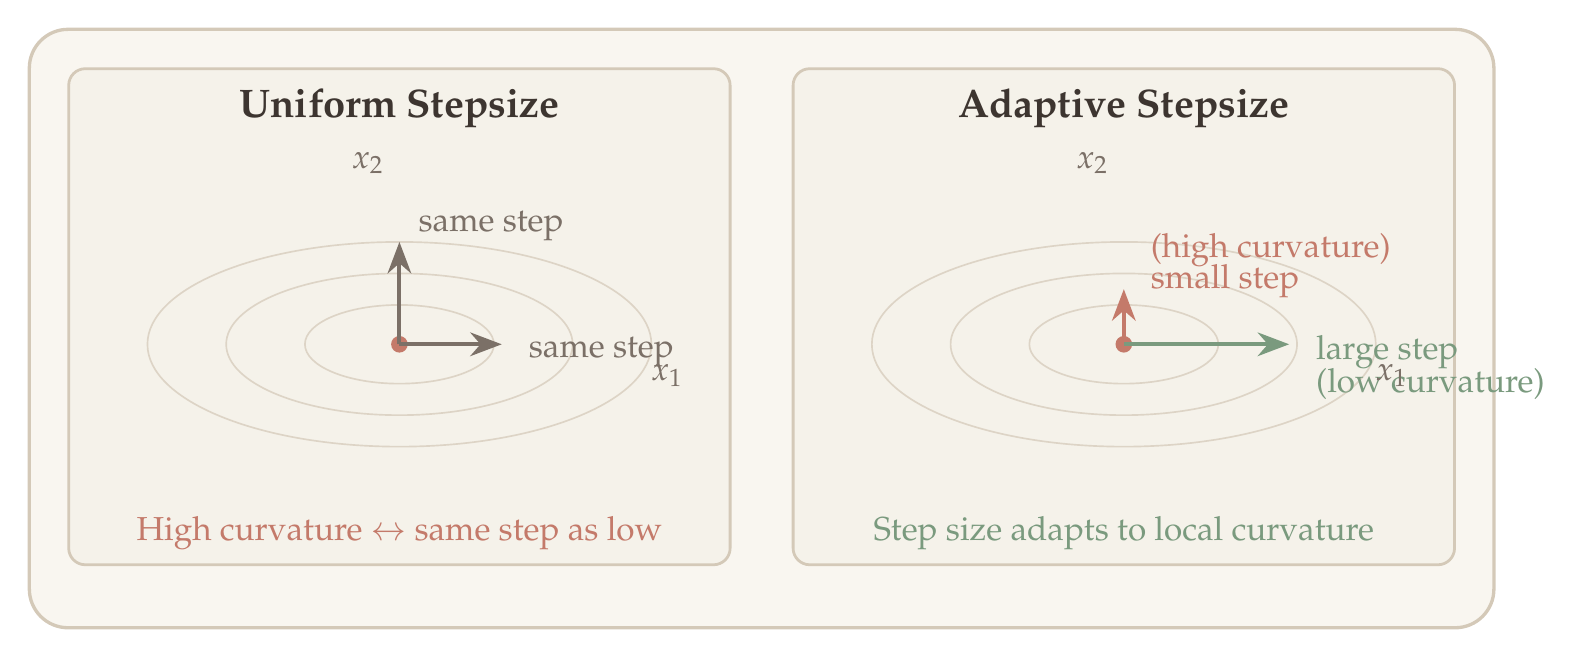
\begin{tikzpicture}[>={Stealth[length=4mm, width=3mm]}, line width=1.5pt]

% Background
\fill[cream, rounded corners=14pt] (-0.3,-0.3) rectangle (18.3,7.3);
\draw[border, line width=1.2pt, rounded corners=14pt] (-0.3,-0.3) rectangle (18.3,7.3);

% Left panel: Uniform Stepsize
\fill[cream!90!border, rounded corners=6pt] (0.2,0.5) rectangle (8.6,6.8);
\draw[border, line width=1pt, rounded corners=6pt] (0.2,0.5) rectangle (8.6,6.8);
\node[text=dkbrown, font=\Large\bfseries] at (4.4,6.3) {Uniform Stepsize};

% Ellipse contours (left)
\draw[border!80, line width=0.6pt] (4.4,3.3) ellipse (3.2cm and 1.3cm);
\draw[border!80, line width=0.6pt] (4.4,3.3) ellipse (2.2cm and 0.9cm);
\draw[border!80, line width=0.6pt] (4.4,3.3) ellipse (1.2cm and 0.5cm);

% Center dot
\fill[terracotta] (4.4,3.3) circle (3pt);

% Uniform arrows (same length in both directions)
\draw[wmgray, ->, line width=1.5pt] (4.4,3.3) -- (5.7,3.3);
\draw[wmgray, ->, line width=1.5pt] (4.4,3.3) -- (4.4,4.6);

% Labels
\node[text=wmgray, font=\large, anchor=west] at (5.9,3.2) {same step};
\node[text=wmgray, font=\large, anchor=west] at (4.5,4.8) {same step};

% Axis labels
\node[text=wmgray, font=\large] at (7.8,2.9) {$x_1$};
\node[text=wmgray, font=\large] at (4.0,5.6) {$x_2$};

% Bottom note
\node[text=terracotta, font=\large] at (4.4,0.9) {High curvature $\leftrightarrow$ same step as low};

% Right panel: Adaptive Stepsize
\fill[cream!90!border, rounded corners=6pt] (9.4,0.5) rectangle (17.8,6.8);
\draw[border, line width=1pt, rounded corners=6pt] (9.4,0.5) rectangle (17.8,6.8);
\node[text=dkbrown, font=\Large\bfseries] at (13.6,6.3) {Adaptive Stepsize};

% Ellipse contours (right)
\draw[border!80, line width=0.6pt] (13.6,3.3) ellipse (3.2cm and 1.3cm);
\draw[border!80, line width=0.6pt] (13.6,3.3) ellipse (2.2cm and 0.9cm);
\draw[border!80, line width=0.6pt] (13.6,3.3) ellipse (1.2cm and 0.5cm);

% Center dot
\fill[terracotta] (13.6,3.3) circle (3pt);

% Short arrow: high curvature (vertical)
\draw[terracotta, ->, line width=1.5pt] (13.6,3.3) -- (13.6,4.0);

% Long arrow: low curvature (horizontal)
\draw[sage, ->, line width=1.5pt] (13.6,3.3) -- (15.7,3.3);

% Labels
\node[text=terracotta, font=\large, anchor=west] at (13.8,4.1) {small step};
\node[text=terracotta, font=\large, anchor=west] at (13.8,4.5) {(high curvature)};
\node[text=sage, font=\large, anchor=west] at (15.9,3.2) {large step};
\node[text=sage, font=\large, anchor=west] at (15.9,2.8) {(low curvature)};

% Axis labels
\node[text=wmgray, font=\large] at (17.0,2.9) {$x_1$};
\node[text=wmgray, font=\large] at (13.2,5.6) {$x_2$};

% Bottom note
\node[text=sage, font=\large] at (13.6,0.9) {Step size adapts to local curvature};

\end{tikzpicture}
\end{document}
